\documentclass[12pt,a4paper]{article}%
\usepackage{makeidx}
\makeindex
\usepackage{bm}
\usepackage{framed} % Easier way to use Framebox
\usepackage{pdfpages} % Import PDF in latex document
\usepackage{listings}
% \usepackage{slashbox}
\usepackage{array}
\usepackage{enumitem}
\usepackage{amsmath, amssymb, amsthm}  % For mathematical symbols
\usepackage{colortbl,color}
\usepackage{xcolor}
\usepackage{auto-pst-pdf}
\usepackage{graphicx,psfrag}
\usepackage{tabularx,array}
\usepackage{booktabs}
\usepackage{multirow}
\usepackage{multicol}
\usepackage[subfigure]{tocloft}
\usepackage[tight]{subfigure}
\usepackage{float,booktabs,threeparttable}
\usepackage{caption}


\usepackage{longtable}
\usepackage{appendix}

\usepackage{pdfpages}
\usepackage{blkarray} %For adding Matrix label on row and column
\usepackage{url}
\usepackage{indentfirst} % indent the first paragraph of new section
\usepackage{titlesec} % change the way \subsubsubsection formats

\def\se{{\rm se}}
%\newcommand{\red}{\color{red}}
\linespread{1.5}  % The linespread is 1.5.

% Numbered theorems, definitions, algorithm and lemmas ======================================================================
\newtheorem{thm}{Theorem}  % Define new theorem.
\newtheorem{alg}{Algorithm}[section]  % Define new algorithm.
\newtheorem{definition}{Definition}
% ===========================================================================================================================

% For writing pseudo code ======================================================================
\usepackage{algorithm}% http://ctan.org/pkg/algorithms
\usepackage{algpseudocode}% http://ctan.org/pkg/algorithmicx
% ===========================================================================================================================

\theoremstyle{definition}
\theoremstyle{plain}
\setcounter{secnumdepth}{5}


\renewcommand{\contentsname}{Table of Contents}
\renewcommand{\listfigurename}{List of Figures}
\renewcommand{\listtablename}{List of Tables}
\renewcommand{\figurename}{\footnotesize Figure}
\renewcommand{\tablename}{\footnotesize Table}
\newcommand{\loflabel}{Figure}
\newcommand{\lotlabel}{Table}
\setlength{\abovecaptionskip}{0pt}


\renewcommand{\cftsecnumwidth}{7em}
\renewcommand{\appendixpagename}{\Large Appendix} % \ctxfb
\renewcommand{\arraystretch}{1.2}

\usepackage{appendix}



%%%%%%%%%%%%

\newtheorem{lma}{\textbf{Lemma}}

% ======================== Set length ========================
\setlength{\columnsep}{1cm}
\setlength\parindent{0pt}
\textheight = 22cm
\textwidth = 16.5cm
\hoffset=-1cm
\footskip=40pt
\renewcommand*{\arraystretch}{0.8}
% ============================================================
% ======================== Paragraph Indent ========================
\setlength{\parindent}{1em}
\setlength{\parskip}{1em}
% ==================================================================
% =============================
% Equation numbering
\numberwithin{equation}{section}
% =============================
% ======================== SubSubSubSection Format ========================
\titleclass{\subsubsubsection}{straight}[\subsection]

\newcounter{subsubsubsection}[subsubsection]
\renewcommand\thesubsubsubsection{\thesubsubsection.\arabic{subsubsubsection}}

\titleformat{\subsubsubsection}
  {\normalfont\normalsize\bfseries}{\thesubsubsubsection}{1em}{}
\titlespacing*{\subsubsubsection}
{0pt}{3.25ex plus 1ex minus .2ex}{1.5ex plus .2ex}
% ==================================================================

\begin{document}
\setcounter{section}{5}
\section{Linear Model Selection and Regularization}
In this chapter we mainly discuss about the methods which multiple linear regression model can be improved. These methods include,
\begin{itemize}
\item Prediction Accuracy: If $p > n$ then there is no longer a unique least squares coefficient estimate: the variance is infinite so the method cannot be used at all. By \textit{constrain} or \textit{shrinking} the estimated coefficients, we can often substantially reduce the variance at the cost of a negligible increase in bias. 
\item Model Interpretability:  Some approaches for automatically performing feature selection or variable selection. That is, for excluding irrelevant variables from a multiple regression model (Lasso).
\end{itemize}

\subsection{\textbf{Subset Selection}}
\subsubsection{\textbf{Best Subset Selection}}
To perform best subset selection, we fit a separate \textit{least squares regression} for each possible combination of the $p$ predictors.
\begin{algorithm}[H]
\caption{Best subset selection}\label{best-subset}
\begin{algorithmic}[1]
\State Let $\mathcal{M}_{0}$ denote the $null$ model, which contain no predictors. This model simply predicts the sample mean for each observations.
\For{$k=1,2,\dots,p$}
\State (a) Fit all ${p}\choose{k}$ models that contain exactly $k$ predictors.
\State (b) Pick the best among these ${p}\choose{k}$ models, and call it $\mathcal{M}_{k}$. Here best is defined as having the smallest RSS, or equivalently largest $R^{2}$
\EndFor
\State Select a single best model from among $\mathcal{M}_{0},\dots,\mathcal{M}_{p}$ using cross-validated prediction error, $C_{p},(AIC),BIC,$ or adjusted $R^{2}$.
\end{algorithmic}
\end{algorithm}

In Algorithm~\ref{best-subset}, Step 2.(b) we select a best model in round $k$ by computing RSS or $R^{2}$. However, a low RSS or a high $R^{2}$ indicates a model with a low training error. In this case we use cross-validated prediction error, $C_{p},(AIC),BIC, adj-R^{2}$ to select among $\mathcal{M}_{0},\dots,\mathcal{M}_{p}$ in order to evaluate our model by computing the test error.

\begin{itemize}
\item Drawbacks
\begin{enumerate}
	\item We have to choose the best model among the $2^{p}$ models, which is computationally expensive.
\end{enumerate}
\end{itemize}

\begin{itemize}
\item Advantages
\begin{enumerate}
	\item The approach guaranties to choose the best model since it evaluates all model combinations.
\end{enumerate}
\end{itemize}

\subsubsection{\textbf{Stepwise Selection}}
\subsubsubsection{Forward Stepwise Selection}

\begin{algorithm}[H]
\caption{Forward Stepwise Selection}\label{forward-stepwise}
\begin{algorithmic}[1]
\State Let $\mathcal{M}_{0}$ denote the $null$ model, which contain no predictors. 
\For{$k=1,2,\dots,p-1$}
\State (a) Consider all $p-k$ models that augment the predictors in $\mathcal{M}_{k}$ with on additional predictor.
\State (b) Choose the best among these $p-k$ models, and call it $\mathcal{M}_{k+1}$. Here best is defined as having smallest RSS or highest $R^{2}$
\EndFor
\State Select a single best model from among $\mathcal{M}_{0},\dots,\mathcal{M}_{p}$ using cross-validated prediction error, $C_{p},(AIC),BIC,$ or adjusted $R^{2}$.
\end{algorithmic}
\end{algorithm}

\begin{itemize}
\item Drawbacks
\begin{enumerate}
	\item For instance, suppose that in a given data set with $p=3$. We already knew that the best one-variable model is $X_{1}$ and the best two-variables model is $X_{2}$ and $X_{3}$. Now, apply the forward stepwise selection and get $X_{1}$ for $\mathcal{M}_{1}$. However, forward stepwise selection will fail in $\mathcal{M}_{2}$, since $X_{1}$ shall be retained in $\mathcal{M}_{2}$ according to the implementation of forward stepwise and this violate what we know of the best two-variable model($X_{2},X_{3}$).
	\item Not guaranteed to yield the best model containing a subset of the $p$ predictors.
\end{enumerate}
\end{itemize}

\begin{itemize}
\item Advantages
\begin{enumerate}
	\item The approach is more efficient than best subset method.
\end{enumerate}
\end{itemize}

\subsubsubsection{Backward Stepwise Selection}
\begin{algorithm}[H]
\caption{Backward Stepwise Selection}\label{backward-stepwise}
\begin{algorithmic}[1]
\State Let $\mathcal{M}_{p}$ denote the $full$ model, which contain all $p$ predictors. 
\For{$k=p,p-1\dots,1$}
\State (a) Consider all $k$ models that contain all but one of the predictors in $\mathcal{M}_{k}$, for a total of $k-1$ predictors.
\State (b) Choose the best among these $k$ models, and call it $\mathcal{M}_{k-1}$. Here best is defined as having smallest RSS or highest $R^{2}$
\EndFor
\State Select a single best model from among $\mathcal{M}_{0},\dots,\mathcal{M}_{p}$ using cross-validated prediction error, $C_{p},(AIC),BIC,$ or adjusted $R^{2}$.
\end{algorithmic}
\end{algorithm}

\begin{itemize}
\item Drawbacks
\begin{enumerate}
	\item $n>p$, otherwise the full model can not be fitted.
	\item Not guaranteed to yield the best model containing a subset of the $p$ predictors.
\end{enumerate}
\end{itemize}

\begin{itemize}
\item Advantages
\begin{enumerate}
	\item The approach is more efficient than best subset method.
\end{enumerate}
\end{itemize}

\subsubsubsection{Hybrid Approaches}~\\
This method is similar to stepwise regression. After adding each new variable, we may also remove any variables that no longer provide an improvement in the model fit (p-value $<$ 0.5).

\subsubsection{\textbf{Choosing the Optimal Model}}
In order to select the best model with respect to test error, we need to estimate this test error. There are two common approaches:
\begin{enumerate}
\item We can indirectly estimate test error by making as adjustment to the training error to account for the bias due to overfitting ($C_{p}$, AIC, BIC, $adj-R^{2}$) .
\item We can directly estimate the test error, using either a validation set approach or a cross-validation approach (k-Fold CV).
\end{enumerate}

\subsubsubsection{\textcolor{blue}{\textbf{$C_{p}$, AIC, BIC, $adj-R^{2}$}}}
\begin{gather*}
C_{p} = \frac{1}{n}(\text{RSS}+2d\hat{\sigma}^{2}) \\
\text{AIC} = \frac{1}{n\hat{\sigma}^{2}}(\text{RSS}+2d\hat{\sigma}^{2})\\
\text{BIC} = \frac{1}{n}(\text{RSS}+\log (n)d\hat{\sigma}^{2})\\
\text{Adjusted } R^{2} = 1-\frac{\text{RSS}/(n-d-1)}{\text{TSS}/(n-1)} 
\end{gather*}

\subsubsubsection{\textcolor{blue}{\textbf{Validation and Cross-Validation}}}
Compares to $C_{p}$, AIC, BIC, and $adj-R^{2}$; validation and cross-validation provides a direct estimate of the test error , and makes fewer assumptions about the true underlying model. 

\subsection{\textbf{Shrinkage Methods}}
In the previous section, our strategy to preform model selection is to fit multiple subsets of models and choose a best one by evaluating measurements such as $C_{p}$ or Cross-Validation error. 
In this section, we tried to shrinks the coefficient estimates or even shrinks towards zero to choose the most preventative predictors. It turns out that shrinking the coefficient estimates can significantly reduce their variance. The two best-known techniques are ridge regression and the lasso.

\subsubsection{\textbf{Ridge Regression}}
The estimation of coefficients is done by introducing a $\ell 2$ regulation in the original RSS model. The $\hat{\beta}^{ridge}_{\lambda}$ of ridge regression takes the form, 
\begin{gather}
\hat{\beta}^{ridge}_{\lambda} = \arg\min_{\beta} \sum\limits_{i=1}^{n} \bigg( y_{i}-\beta_{0}- \sum\limits_{j=1}^{p}\beta_{j}x_{ij} \bigg)^{2} + \lambda \sum\limits_{j=1}^{p}\beta_{j}^{2}
\label{ridgeFormula}
\end{gather}

Another way to describe ridge regression,
\begin{equation}
\begin{aligned}
\begin{split}
& \underset{\beta}{\text{minimize}} & & Z = \sum\limits_{i=1}^{n} \bigg( y_{i}-\beta_{0}- \sum\limits_{j=1}^{p}\beta_{j}x_{ij} \bigg)^{2} \\
& \text{subject to} 				& & \\
& & & \sum\limits_{j=1}^{p}\beta_{j}^{2} \leq s
\end{split}
\end{aligned}
\label{lasso}
\end{equation}

It's simple to get the closed form of $\hat{\beta}^{ridge}_{\lambda}$ by first order differential,
\begin{gather*}
\hat{\beta}^{ridge}_{\lambda} = (\lambda \mathbf{I}_{D} + \mathbf{X}^{T} \mathbf{X})^{-1} \mathbf{X}^{T} \mathbf{y}
\end{gather*}

\begin{figure}[H]
\centering
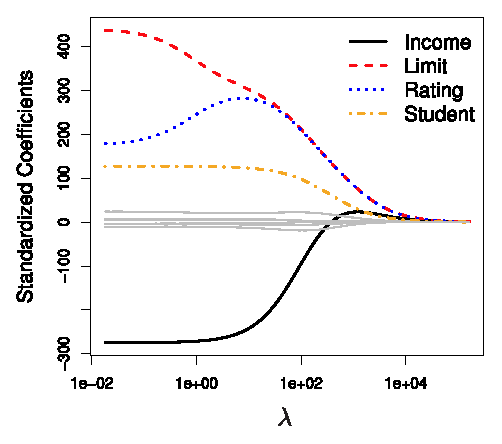
\includegraphics[scale=1]{images//6_4.eps}
\\~\\
\caption{ }\label{ridgeRegression}
\end{figure}

Figure~\ref{ridgeRegression} shows an illustration of the ridge regression optimization from \eqref{ridgeFormula}. When $\lambda=0$, the penalty term has no effect, and ridge regression will produce the least squares estimates. However, as $\lambda \rightarrow \infty$, the impact of the shrinkage penalty grows, and the ridge regression coefficient estimates will approach zero. 

\subsubsubsection{\textcolor{blue}{Scale equivariant}}
Consider the following scenario,
\begin{enumerate}
\item First, fit $X_{j}$ by least square errors. This will give us $\hat{\beta}_{j}$
\item Second, we multiply $X_{j}$ by a constant $c$ and fit the parameters by least square errors again. Now, the $\hat{\beta}_{j}$ will takes the transformation as the original $\hat{\beta}_{j} \times \frac{1}{c}$
\end{enumerate}

In other words, regardless of how $X_{j}$ is scaled, $X_{j}\hat{\beta}$ will remain the same. Since $X_{j}$ are in different scale, the value for $\beta_{j}$ range widely. 
This will impact the ridge penalty term and lead the penalty to a high variance. Ridge regression regularize the linear regression by imposing a penalty on the size of coefficients. Thus the coefficients are shrunk toward zero and toward each other. But when this happens and if the independent variables does not have the same scale, the shrinking is not fair. Two independent variables with different scales will have different contributions to the penalized terms, because the penalized term is a sum of squares of all the coefficients. To avoid such kind of problems, very often, the independent variables are centred and scaled in order to have variance 1. In this case, we should standardizing predictors before we apply ridge regression. The standardizing formula takes the form,
\begin{gather*}
\tilde{x}_{ij} = \frac{x_{ij}}{\sqrt{\frac{1}{n}\sum\limits^{n}_{i=1} (x_{ij}-\bar{x}_{j})^{2}}}
\end{gather*}
Assume our test data are represent as $z_{ij}$, the standardizing of test data takes the form,
\begin{gather*}
\tilde{z}_{ij} = \frac{z_{ij}}{\sqrt{\frac{1}{n}\sum\limits^{n}_{i=1} (x_{ij}-\bar{x}_{j})^{2}}}
\end{gather*}

\subsubsection{\textbf{Lasso}}
As with ridge regression, the lasso shrinks the coefficient estimates towards zero. In other words, Lasso also performs variable selection when $\lambda$ is sufficiently large. 

Another way to describe Lasso:
\begin{equation}
\begin{aligned}
\begin{split}
& \underset{\beta}{\text{minimize}} & & Z = \sum\limits_{i=1}^{n} \bigg( y_{i}-\beta_{0}- \sum\limits_{j=1}^{p}\beta_{j}x_{ij} \bigg)^{2} \\
& \text{subject to} 				& & \\
& & & \sum\limits_{j=1}^{p}|\beta_{j}| \leq s
\end{split}
\end{aligned}
\label{lasso}
\end{equation}

When $p=2$, then \eqref{lasso} indicates that the lasso coefficient estimates have the smallest RSS out of all points that lie within the diamond defined by $|\beta_{1}|+|\beta_{2}| \leq s$. 
The illustration of the formula in Figure~\ref{lassoOpti}. \\

We can think of a set of coefficients $\boldsymbol\beta$ are constrained by $s$ from \eqref{lasso}. 
So, if $s$ is extremely large, we will get the least square estimates while the constraint is not very restrictive.
On the other hand, if $s$ is approximately to zero, some of the estimates we get will be zero, since the constraint is highly restrictive. 

%==================================================================================================================================================================================================================

\subsubsubsection{\textcolor{blue}{The Variable Selection Property of the Lasso}}
\begin{figure}[H]
\centering
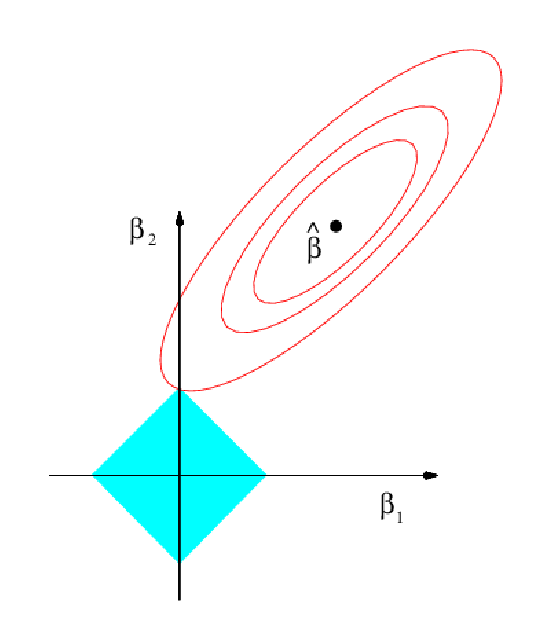
\includegraphics[scale=0.8]{images//6_7.eps}
\\~\\
\caption{ }\label{lassoOpti}
\end{figure}

The least squares estimates is marked as $\hat{\beta}$, while the blue diamond represent the lasso constraints. 
If $s$ is sufficiently large, then the constraint regions will cover $\hat{\beta}$, and the lasso estimates will be the same as $\hat{\beta}$. 

The ellipses that are centred around $\hat{\beta}$ represent regions of constant RSS. As the ellipses expand away from $\hat{\beta}$, the RSS increases. 
The lasso constraint has corners at each of the axes, so the ellipse will often intersect the constraint region at an axis. When this occurs, one of the coefficients will equal zero. 
In higher dimensions, many of the coefficient estimates may equal zero simultaneously. 
In Figure~\ref{lassoOpti} , the intersection occurs at $\beta_{1}=0$, so the resulting model will only include $\beta_{2}$.

%==================================================================================================================================================================================================================

\subsubsubsection{\textcolor{blue}{A simple case for the Lasso}}
Assume we are performing regression without an intercept, $n=p$ and $\mathbf{X}$ a diagonal matrix with 1's on the diagonal and 0's in all off-diagonal elements.
With these assumptions, the least squares takes for form,
\begin{equation}
\hat{\beta} = \arg\min_{\beta} \sum\limits_{j=1}^{p} (y_{j}-\beta_{j})^{2}
\end{equation}


In this case, the least squares estimator is given by,
\begin{equation*}
\hat{\beta}_{j} = y_{j}
\end{equation*}

In this setting, the lasso amounts to finding the coefficients such that
\begin{equation}
\hat{\beta}_{\lambda}^{lasso} = \arg\min_{\beta} \sum\limits_{j=1}^{p} (y_{j}-\beta_{j})^{2} + \lambda \sum\limits_{j=1}^{p} |\beta_{j}|
\end{equation}

One can show that
\begin{equation}
\frac{\partial}{\partial \beta_{j}} \text{RSS} = -2(y_{j}-\beta_{j})
\end{equation}

Adding in the penalty term, we find that the subderivative is given by
\begin{align*}
\frac{\partial}{\partial \beta_{j}} f(\boldsymbol{\beta}) &= -2(y_{j}-\beta_{j}) + \lambda \frac{\partial}{\partial \beta_{j}} |\beta_{j}| \\
													      &= \left\{
\begin{array}{ll}
-2(y_{j}-\beta_{j})+\lambda & \mbox{if } \beta_{j} > 0, \\
{[}-2y_{j}-\lambda,-2y_{j}+\lambda{]} & \mbox{if } \beta_{j} = 0, \\
-2(y_{j}-\beta_{j})-\lambda & \mbox{if } \beta_{j} < 0,
\end{array} \right.
\end{align*}

Depending on the value of $y_{j}$ , the solution to $\frac{\partial}{\partial \beta_{j}} f(\boldsymbol{\beta}) =0$ can occur at 3 different values of $\beta_{j}$ , as follows:
\begin{equation*}
\beta_{j} = \left\{
\begin{array}{ll}
y_{j}-\frac{\lambda}{2}   & \mbox{if }  y_{j} > \frac{\lambda}{2}, \\
 0 & \mbox{if } -\frac{\lambda}{2}<y_{j}< \frac{\lambda}{2}, \\
y_{j}+\frac{\lambda}{2}   & \mbox{if } y_{j} < -\frac{\lambda}{2},
\end{array} \right.
\end{equation*}

If $\lambda = 1$, then the two dimensional figure of $\beta_{j}$ vs. $y_{j}$,
\begin{figure}[H]
\centering
\psfrag{A}{\large $y_{j}$}
\psfrag{B}{\large $\beta_{j}$}
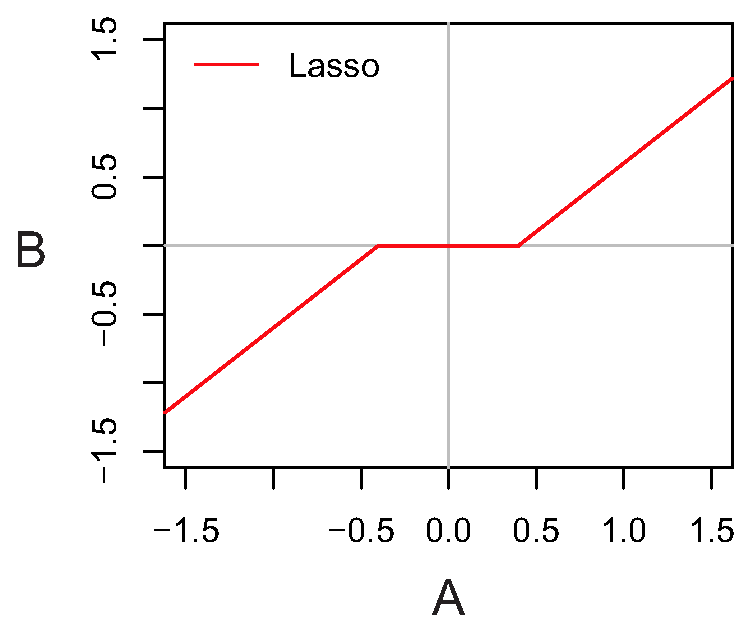
\includegraphics[scale=0.8]{images//6_10.eps}
\\~\\
\caption{ }\label{softThresholding}
\end{figure}

%==================================================================================================================================================================================================================
\subsubsubsection{$\ell 1$ regularization: algorithms}
Now, we derive the general form of lasso, the RSS,
\begin{equation}
\text{RSS} =  \sum\limits_{i=1}^{n} (y_{i}- \sum\limits_{j=1}^{p} \beta_{j} x_{ij})^{2}
\end{equation}

The partial derivative of $\beta_{j}$ on RSS, 
\begin{align*}
\frac{\partial}{\partial\beta_{j}} \text{RSS} &=  2 \sum\limits_{i=1}^{n} \bigg(y_{i}- \sum\limits_{j=1}^{p} \beta_{j} x_{ij}\bigg) (-x_{ij}) \\
 											  &=  2 \sum\limits_{i=1}^{n} \bigg(y_{i} - \sum\limits_{z \neq j}^{p} \beta_{z} x_{iz} -  \beta_{j}x_{ij} \bigg) (-x_{ij}) \\
 											  &=  2 \sum\limits_{i=1}^{n} x_{ij}^{2} \beta_{j} - 2\sum\limits_{i=1}^{n} x_{ij}(y_{i} - \sum\limits_{z \neq j}^{p} \beta_{z} x_{iz}) \\
 											  &=  a_{j}\beta_{j} - c_{j} \\
        							  a_{j}   &=  2 \sum\limits_{i=1}^{n} x_{ij}^{2}  \\
                                      c_{j}   &=  2\sum\limits_{i=1}^{n} x_{ij}(y_{i} - \sum\limits_{z \neq j}^{p} \beta_{z} x_{iz})
\end{align*}
where $z$ is the index represent the coefficients without $j$. Adding in the penalty term, we find that the subderivative is given by,
\begin{align*}
\frac{\partial}{\partial \beta_{j}} f(\boldsymbol{\beta}) &= (a_{j}\beta_{j} - c_{j}) + \lambda \frac{\partial}{\partial \beta_{j}} |\beta_{j}| \\
													      &= \left\{
\begin{array}{ll}
(a_{j}\beta_{j} - c_{j})-\lambda & \mbox{if } \beta_{j} < 0,\\
{[} -c_{j}-\lambda , -c_{j}+\lambda {]} & \mbox{if } \beta_{j} = 0, \\
(a_{j}\beta_{j} - c_{j})+\lambda & \mbox{if } \beta_{j} > 0, 
\end{array} \right.
\end{align*}

Depending on the value of $c_{j}$ , the solution to $\frac{\partial}{\partial \beta_{j}} f(\boldsymbol{\beta}) =0$ can occur at 3 different values of $\beta_{j}$ , as follows:
\begin{equation*}
\hat{\beta}_{j} = \left\{
\begin{array}{ll}
\frac{c_{j}+\lambda}{a_{j}}   & \mbox{if } c_{j} < -\lambda, \\
 0 & \mbox{if } -\lambda < c_{j} < \lambda , \\
\frac{c_{j}-\lambda}{a_{j}}  & \mbox{if }  c_{j} > \lambda,
\end{array} \right.
\end{equation*}

We can write this as follows:
\begin{equation*}
\hat{\beta}_{j} = \text{soft}(\frac{c_{j}}{a_{j}};\frac{\lambda}{a_{j}})
\end{equation*}

where
\begin{equation*}
\text{soft}(a;\delta) \triangleq  \text{sign}(a) (|a|-\delta)_{+}
\end{equation*}

Note that $x_{+} = \text{max}(x, 0)$ is the positive part of $x$ and the definition of sign,
\begin{equation*} 
\text{sign}(x) = 
\left\{
\begin{array}{ll}
-1  & \mbox{if } x < 0, \\
 0  & \mbox{if } x = 0, \\
 1  & \mbox{if } x > 0,
\end{array} \right.
\end{equation*}

\subsubsubsection{Shooting algorithm}
\begin{algorithm}[H]
\caption{Shooting algorithm}\label{ShootingAlgorithm}
\begin{algorithmic}[1]
\State Initialize $\boldsymbol{\beta} = (\mathbf{X}^{T}\mathbf{X} + \lambda \mathbf{I})^{-1}\mathbf{X}^{T}\mathbf{y} ;$
\Repeat
\For{$j=1,\dots ,D$}
\State $a_{j} = 2 \sum\limits_{i=1}^{n} x_{ij}^{2}$
\State $c_{j} = 2\sum\limits_{i=1}^{n} x_{ij}(y_{i} - \boldsymbol{\beta}^{T}\mathbf{x}_{i}+\beta_{j}x_{ij})$
\State $\beta_{j} = \text{soft}(\frac{c_{j}}{a_{j}};\frac{\lambda}{a_{j}})$
\EndFor
\Until{calculate loss function to check converged;}
\end{algorithmic}
\end{algorithm}

The problem with Shooting Algorithm is that it only updates one variable at a time, so can be slow to converge. 
LARS can compute $\hat\beta(\lambda)$ for all possible values of $\lambda$ in an efficient manner. To see more reference on LARS and lasso. \footnotemark
\footnotetext{Lasso for logistic regression (see Yuan et al. 2010). And see (Schmidt et al. 2009; Yuan et al. 2010; Yang et al. 2010) for some recent surveys }


%==================================================================================================================================================================================================================

\end{document}
